%%%%%%%%%%%%%%%%% your_thesis_eng.tex %%%%%%%%%%%%%%%%%
%
% This is the template file for ORM 2016 proceedings.
%
% Please, fill in following the directions below.
%
%%%%%%%%%%%%%%%%%%%%%%%%%%%%%%%%%%%%%%%%%%%%%%%%%%%%%%%

\newcommand{\No}{No.}

\Title[%
% Insert here the acknowledgements of grants and/or any other
% information you wish to appear as a footnote, or leave this
% field blank.
The reported study was funded by RFBR according to the research project \No 16-01-00353a.%
]
{%
% Insert your title here
Multistage Bidding Model with Elements of Bargaining. Extension for a Countable State Space%
}
{%
% Insert the authors' names here
A.I.~Pyanykh%
}
{%
% Insert your institution here
Moscow State University%
}
{%
% Insert your city here
Moscow%
}
{%
% Insert your country here
Russia%
}

% Insert your thesis here.
% The entire submission should not exceed 3 pages if you plan a publication in conference proceedings.
%
% ATTENTION: Using 'thebibliography' environment is not allowed.
% Use 'references_eng' environment below to format the list of references.
% Please note that the latter environment does not provide automatic
% citation facilities. Cite manually using square brackets,
% e.g., [1], [2, 3], [4--6].
%
We consider a simplified model of a financial market with two players bidding
for one unit of a risky asset (a share) for $n \leq \infty$ consecutive stages.
Player 1 (an insider) is informed about the liquidation price $s$ of the asset
while Player 2 knows only its probability distribution $p$. At each
stage players place integral bids. The higher bid wins and a share is transacted
to the winning player. Each player aims to maximize the value of her final
portfolio.

A model where the price $s$ has only two possible values $\{0, m\}$ is
considered in [1]. It is reduced to a zero-sum game $G_n(p)$ with
incomplete information on one side as in Aumann, Maschler [2]. In this model
uninformed Player 2 uses the history of Player 1's moves to update the posterior
probabilities over the liquidation price. Thus, Player 1 should find a strategy
controlling posterior probabilities in such a way that allows her to use the
private information without revealing too much of it to Player 2. The main
results in [1] are explicit optimal strategies and the value of the game
$G_\infty(p)$. In [3] the model is extended so that the liquidation
price can take any value $s \in S = \mathbb{Z}_+$ according to a probability
distribution $p = (p_0, p_1, \ldots)$. It is shown that when
$\mathbb{D} p < \infty$ a game $G_\infty(p)$ is properly
defined. For this game the value and optimal players strategies are found.

In both [1] and [3] the transaction price equals to the highest bid. Instead we
could consider a transaction rule proposed in [4], and define a price at which
the asset is transacted equal to a convex combination of proposed bids with some
coefficient $\beta \in [0, 1]$. A model with such transaction rule and two
possible values of the liquidation price is analyzed in [5]. Here these results
are futher extended for the case of a countable state space.

Formally the model is defined as follows. At stage 0 a chance move chooses a
state of nature $s \in S$ according to the distribution $p$. At each stage $t =
\overline{1,n}$ players make bids $i_t \in I, j_t \in J$ where $I = J =
\mathbb{Z}_+$. Denoting $\overline{\beta} = 1-\beta$ a stage payoff in state $s$
equals to
\begin{equation*}
  a^s(i, j) =
  \begin{cases}
    \overline{\beta} i + \beta j - s, &\; i < j,\\
    0, &\; i = j,\\
    s - \beta i - \overline{\beta} j, &\; i > j.
  \end{cases}
\end{equation*}

Player 1's strategy is a sequence of actions $\sigma = (\sigma_1, \ldots,
\sigma_n)$ where $\sigma_t:~S \times I^{t-1} \rightarrow \Delta(I)$ is a mapping
to the set of probability distributions $\Delta(I)$ over $I$. That is, at each
stage Player 1 randomizes his bids depending on the history up to stage $t$ and
the liquidation price $s$. Similarly, Player 2's strategy $\tau = (\tau_1,
\ldots, \tau_n)$ where $\tau_t:~J^{t-1} \rightarrow \Delta(J)$. Player 1's
payoff then defined as $K_n(p, \sigma, \tau) = \mathbb{E}_{(p, \sigma, \tau)}
\sum_{t=1}^n a^s(i_t,j_t)$. Player 2's payoff equals to $-K_n(p, \sigma, \tau)$.

Following [3], Player 1's strategy $\sigma$ in $n$--stage game can be
represented as a pair $(\sigma_1, \sigma(i))$ where $\sigma_1$ is a one stage
action and $\sigma(i)$ is a strategy in $(n-1)$--stage game dependent on the
actual first bid. Similarly Player 2's strategy $\tau$ can be represented as a
pair $(\tau_1, \tau(i))$. Denoting $q = (q_0, q_1, \ldots)$ a marginal
distribution of the first bid, and $p(i) = \{p(0 | i), p(1, i), \ldots\}$ -- a
posterior distribution of the liquidation price given a bid $i$, the following
recursive formula holds
\begin{equation*}
  K_n(p, \sigma, \tau) = K_1(p, \sigma_1, \tau_1) +
  \sum_{i \in I} q_i K_{n-1}(p(i), \sigma(i), \tau(i)).
\end{equation*}
Thus to define a strategy in $G_n(p)$ it is suffice to define a stage action for
any posterior probability $p$. Let's define a pure strategy $\tau^k$ as
\begin{gather*}
  \tau_1^k = k, \quad
  \tau_t^k(i_{t-1}, j_{t-1}) =
  \begin{cases}
    j_{t-1}, &\; i_{t-1} < j_{t-1},\\
    j_{t-1}, &\; i_{t-1} = j_{t-1},\\
    j_{t-1}, &\; i_{t-1} > j_{t-1}.
  \end{cases}
\end{gather*}
It can be shown that for $p$ such that $\mathbb{E} p = k - 1 + \beta + \xi, \;
\xi \in [0, 1)$ Player 2 can guarantee a payoff not more than $H^\infty(p) =
\mathbb{D} p + \beta\overline{\beta} -\xi(1-\xi)$. Function $H^\infty(p)$ is
piecewise linear with breakpoints at $p \in \Theta(k + \beta)$ where $\Theta(x)
= \{p: \mathbb{E} p = x\}$ and domains of linearity $\Lambda(k -
\overline{\beta}, k + \beta)$ where $\Lambda(x, y) = \{p: x \leq \mathbb{E}p
\leq y \}$.

Given $\sigma_1 = \{q_1, p_1(i)\}$ and $\sigma_2 = \{q_2, p_2(i)\}$ are two
first-stage actions and $p = \lambda p_1 + (1-\lambda)p_2$, it can be shown that
a first-stage action $\sigma$ with $q_i = \lambda q_{1,i} + (1-\lambda) q_{2,i}$
and $p(s|i) = (\lambda q_{1,i} p_1(s|i) + (1-\lambda) q_{2,i} p_2(s|i))/q_i$
guarantees Player 1 a payoff of at least $L_n(p, \sigma) = \lambda L_{n-1}(p_1,
\sigma_1) + (1-\lambda) L_{n-1}(p_2, \sigma_2)$. Since every $p$ can be
represented as a convex combination of distributions taking only 2 different
values it is suffice to show that $H^\infty(p^{k+\beta}(r, l)) =
B_\infty(p^{k+\beta}(r, l))$ to prove that $H^\infty(p) = B_\infty(p)$ for all
$p$.

An optimal strategy for $p^x(0, m)$ is described in [5]. Adjusting it for
$p^{k+\beta}(l, r)$ gives us $L_\infty(p^{k+\beta}(l, r)) = ((r - k - \beta)(k -
l + \beta) + \beta(1-\beta))/2 = H_\infty(p^{k+\beta}(l, r))$. Thus the game
$G_\infty(p)$ has a value $V_\infty(p) = H_\infty(p)$.

It is important to note that Player 1's strategy described above is properly
defined only for $\beta \in (0, 1)$. In case of $\beta \in \{0, 1\}$ one should
use strategies described in [3].

% Insert your figure, if needed.
% \begin{figure}[!h]
%   \centering
%   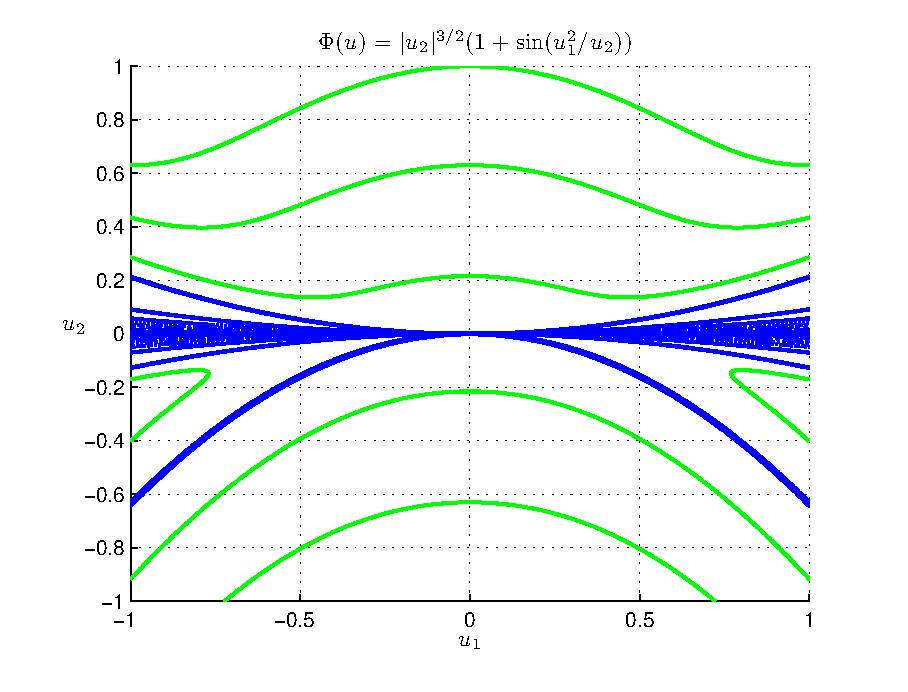
\includegraphics[width=0.7\maxpicturewidth]{your_figure.eps}
%   \center{Fig.~1. Your caption.}
% \end{figure}

\begin{references_eng}
% Insert your list of references here. The order of items in the list must
% agree with the order of their appearance in the text of your thesis.
% Use the '\url' command for citing url-s: e.g., \url{http://http://www.mathopt.org/}.

\item % Reference No. 1
  Domansky~V. Repeated games with asymmetric information and random price fluctuations at finance markets // International Journal of Game Theory. 2007. V.~36, \No~2. P.~241--257.

\item
  Aumann R.J., Maschler M.B. Repeated Games with Incomplete Information. Cambridge, Massachusetts: The MIT Press, 1995.

\item % Reference No. 2
  Domansky~V.C., Kreps~V.L. Game Theoretic Bidding Model: Strategic Aspects of Price Formation at Stock Markets // The Journal of the New Economic Association. 2011. V.~11. P.~39--62.

\item
  Chatterjee~K., Samuelson W. Bargaining under incomplete information //
  Operations Research. 1983. V.~31, \No 5. P.~835--851.

\item
  P'yanykh~A.I. A Multistage Exchange Trading Model with Asymmetric Information and Elements of Bargaining // Moscow University Computational Mathematics and Cybernetics. 2016. V.~40, \No~1. P.~35--40.
% ...

\end{references_eng}

%%%%%%%%%%%%%%%%%%%%%%%%%%%%%%%%%%%%%%%%%%%%%%%%%%%%%%%

%%% Local Variables:
%%% mode: latex
%%% TeX-master: "main"
%%% End:
